
\documentclass[12pt]{article}
%\documentclass[smallextended,numbook]{svjour3}

\usepackage[english]{babel}
\usepackage[utf8x]{inputenc}
\usepackage{pdfpages}
\usepackage{amsfonts,dsfont}
\usepackage{amsmath}
\usepackage{amssymb}
\usepackage{amsthm} %commenter pour style MP
\usepackage{bm}
\usepackage{natbib}
\usepackage{hyperref}
\usepackage{algorithm2e}
\usepackage{enumitem}
\usepackage[capitalise]{cleveref}
%\usepackage[capitalise,poorman]{cleveref}

\setlength {\marginparwidth }{2cm}
\usepackage{todonotes}
\usepackage[all]{xy} 

\makeatletter \let\cl@part\relax \makeatother

%\usepackage[top=1cm, bottom=1cm, left=1cm, right=1cm]{geometry}
\usepackage[top=2cm, bottom=2cm, left=2cm, right=2cm]{geometry}
\usepackage{xcolor}
\usepackage{tikz}
\usetikzlibrary{calc}
\usetikzlibrary{intersections}
\tikzset{offset/.style={to path={%
    -- ($(\tikztostart)!#1cm!(\tikztotarget)$)}},
         offset/.default=1}
\tikzset{>=latex}


\renewcommand{\thesection}{\Alph{section}}
\usepackage{pgfplots}

\newcommand{\mf}[1]{\begin{color}{brown}\texttt{MF:#1}\end{color}}

\newcommand{\TODO}{\begin{color}{red}TODO\end{color}}

\newcommand{\tco}{tCO_2eq}

\newcommand{\ques}[1]{\begin{enumerate}[resume]
\item  #1
\end{enumerate}}

\newcommand{\rep}[1]{\textit{Réponse :} #1 \\}
\renewcommand{\rep}[1]{ }






\usepackage{subcaption}
%\usepackage[colorinlistoftodos,bordercolor=orange,backgroundcolor=orange!20,linecolor=orange,textsize=scriptsize]{todonotes}


%% Theorems
\newtheorem{hypo}{Assumption}
\Crefname{hypo}{Assumption}{Assumptions}

\newtheorem{theorem}{Theorem}
\newtheorem{lemma}[theorem]{Lemma}
\newtheorem{remark}[theorem]{Remark}
\newtheorem{cor}[theorem]{Corollary}
\newtheorem{prop}[theorem]{Proposition}
\newtheorem{defi}[theorem]{Definition}
\newtheorem{conj}{Conjecture}
\newtheorem{nota}{Notation}
\theoremstyle{remark}
\newtheorem{exa}{Example}


\def\NN{\mathbb{N}}


\title{TD \\Modèle 
DICE (Dynamic Integrated Climate Economy) \\
de Nordhaus simplifié }

\author{Maël Forcier}


\begin{document}
\maketitle


\section{Modélisation économique}

Le modèle DICE, imaginé en 1992 par Nordhaus, est un modèle de macroéconomie qui étudie l'évolution de l'économie mondiale.
Le modèle est dynamique, les variables non-constantes seront indicés par les pas de temps $n$.
La variable principale est le capital, noté $K_n$, c'est-à-dire la valeur en \$ de tous les biens matériels ou immatériels dans le monde.
Le produit intérieur brut (PIB) en \$ noté $Q_n$ est la somme de tous les revenus annuels d'une économie.
La consommation notée $C_n$ est la somme en \$ de tous les biens et services perissables créés puis utilisés pendant une année.
L'investissement en \$ noté $I_n$ est l'ensemble des valeurs crées sur une année qui participent durablement au capital.

\begin{enumerate}
\item On suppose que le PIB dépend uniquement de la consommation et l'investissement. Proposer une équation reliant $Q_n$, $C_n$ et $I_n$.
\end{enumerate}
\rep{ $Q_{n}=C_n + I_n$ }
\begin{enumerate}[resume]
\item  Le capital accumulé se déprécie à un taux $\delta$ qui le fait diminuer entre chaque étape, mais l'investissement permet de générer du nouveau capital. Proposer une équation dite de dynamique reliant $K_{n}$, $K_{n-1}$, $I_n$ et $\delta$.
\end{enumerate}
\rep{ $K_{n}=(1-\delta)K_{n-1}+I_n$ }

L'équation de Cobb-Douglas, classique en macroéconomie pour étudier la croissance, fait l'hypo-thèse que le PIB $Q_n$ est égal au produit $AK_n^\gamma L_n^{1-\gamma}$ où $A$ est appelé le facteur de productivité, $\gamma$ l'élasticité du capital et $L_n$ le travail, souvent approximé comme étant égal à la population. Pour simplifier, nous négligerons l'effet de la population et prendrons une élasticité du capital de $\gamma=1$. Pour prendre en compte le réchauffement climatique, Nordhaus suppose que le PIB $Q_n$ est également proportionnel à un facteur $\Omega_n$ qui modélise les effets du climat. 
\ques{  Proposer une équation de Cobb-Douglas simplifiée (sans le travail) et qui prend en compte le climat en reliant $Q_{n}$, $A$,$\Omega_n$ et $K_{n}$.
}
\rep{ $Q_{n}=A \Omega_n K_n$ }
Selon Eurostat, l'investissement représente environ 23 \% du PIB en Europe et cette part est stable entre 2005 et 2009. Pour simplifier, on considèrera que l'investissement représente un quart du PIB : $I_n=Q_n/4$.
\ques{Avec cette hypothèses, simplifier les équations pour obtenir une relation entre $K_n$, $K_{n-1}$, $A$, $\Omega_n$ et $\delta$. \label{ques:dynamique_K_1}}
\rep{\begin{equation*} K_n=\frac{1- \delta}{1- \frac{A\Omega_n}{4}} K_{n-1}\end{equation*}}


\section{Modélisation de l'effet du climat}

Nous allons maintenant modéliser les dégâts causées par le réchauffement climatique. Nordhaus choisit de de modéliser $\Omega_n$ comme le rapport d'un accroissement du à un taux noté $\alpha_n$ modélisant les coûts d'investissement dans les technologies bas carbone et à une dépréciation du à un taux $d_n$ modélisant les dommages que le réchauffement climatique cause sur le PIB :
\begin{equation*}
\Omega_n=\frac{1-\alpha_n}{1+d_n}
\end{equation*}
On note $T_n$ l'augmentation de la température en °C par rapport à l'ère préindustrielle soit 1850.
En s'appuyant sur quelques papiers économiques de son époque, Nordhaus fait l'hypothèse qu'un réchauffement climatique de 3°C fait baisser le PIB de 1,33 \%. 
Constatant que les dégats sur le PIB ne sont pas linéaires avec la température, Nordhaus suppose également que les dégâts évoluent comme une fonction dépendant linéairement du carré de la température.


\ques{  Avec ces hypothèses, proposer une relation entre $d_n$ et $T_n$. \label{ques:degat_nordhaus}
}
\rep{ \begin{equation*}
d_{n}=0,0133(\frac{T_n}{3})^2 \end{equation*}
}

On veut maintenant modéliser l'effet des émissions de gaz à effet de serre sur la température. On note $M_n$ le total d'émissions cumulées dans l'atmosphère en $G\tco$. Pour rappel, le GIEC présente dans le graphique ci-dessous le lien entre les émissions cumulées et l'augmentation de la Température.
\begin{figure}[h]
\centering
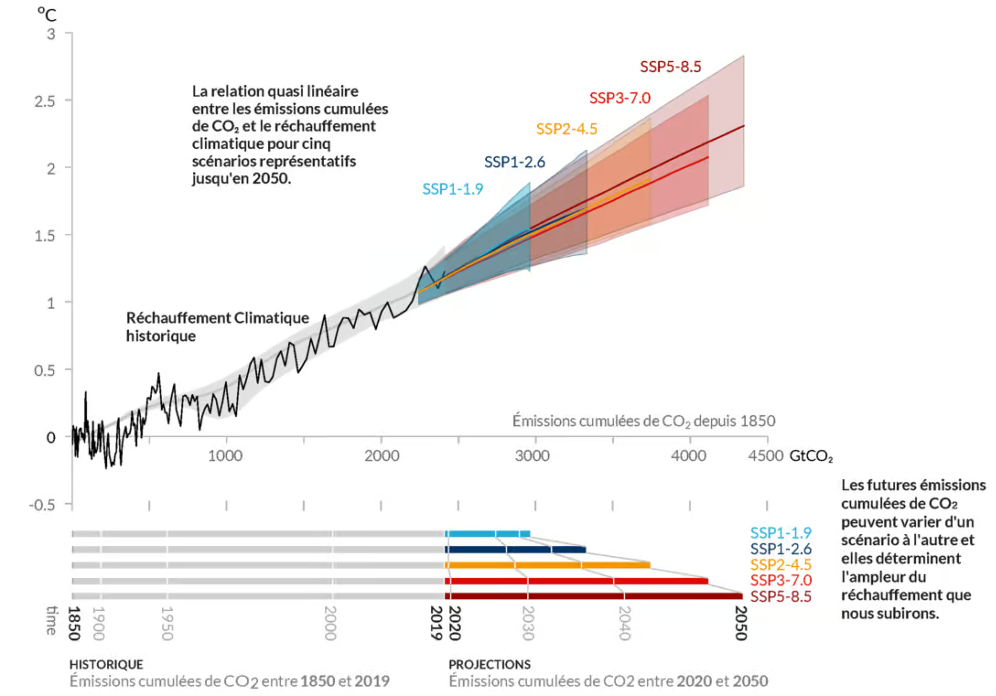
\includegraphics[scale=0.4]{images/Lien_GES_temperature.png}
\end{figure}


\ques{A partir du graphique ci-dessous, proposer une relation simple entre $T_n$ et $M_n$}
\rep{\begin{equation*} T_n= \frac{M_n}{2000}\end{equation*}}

\ques{On commencera le modèle en 2000. On fixe alors la température $T_0$ comme la température de 2000 et les émissions cumulées $M_0$ comme celles de 2000.
Proposer des valeurs arrondies de $T_0$ et $M_0$, cohérentes avec l'équation précédente.}
\rep{$T_0 = 0,8$ °C, $M_0 = 1600$ G$\tco$}

On note $E_n$ les emissions à chaque pas de temps (flux), là où $M_n$ constitue le stock.
Les émissions évoluent selon une dynamique particulière entre les océans, l'atmosphère et le rayonnement solaire, qui suit les équations de la thermodynamique et de la mécanique des fluides.
Pour simplifier, on considérera que toutes les émissions restent dans l'atmosphère.
\ques{ Avec ces hypothèses simplifiées, proposer une équation entre $M_n$, $M_{n-1}$ et $E_n$.}
\rep{$M_n =M_{n-1} +E_n$}

Enfin, Nordhaus considère une variable $\mu_n$ appelé "taux de contrôle des émissions".
Elle modélise l'effort des gouvernements pour contrôler les émissions de l'économie mondiale :
\begin{equation*}
E_n=(1-\mu_n)\sigma Q_n
\end{equation*}
Avec $\sigma$ une constante qui représente le facteur d'émission du PIB dans un scénario sans contrôle $\mu_n=0$. 
Dans le cas $\mu_n=1$, le contrôle est total, on n'émet pas de gaz à effet de serre.
\ques{Exprimer $T_n$ en fonction de $\sigma$, $\mu_1, \cdots, \mu_n$ et $Q_1, \cdots ,Q_n$}.
\rep{\begin{equation*}T_n= T_0+\frac{\sigma}{2000} \sum_{k=1}^n (1-\mu_k) Q_k  \end{equation*}}

Enfin, Nordhaus estime que le coût de l'investissement $\alpha_n$ dans les technologies bas carbone s'exprime comme $0,0686 \mu_n^{2,887}$. Pour simplifier, on pose $\alpha_n = 0,05\mu_n^3$. Ceci donne 
\begin{equation*}
\Omega_n = \frac{1-0,05\mu_n^3}{1+0,0133 (\frac{T_n}{3})^2}
\end{equation*}

\section{Scénario contrôle total}
On considère dans cette partie un scénario où l'on décide de contrôler totalement les émissions : $\forall n, \mu_n=1$.
\ques{Estimer à l'aide du graphique la température moyenne au début de l'expérience Calculer la température à tout temps $n$ en fonction de la température $T_0$ au début de l'expérience. }
\rep{$\forall n, T_n =T_0 = 0,8$°C.}

\ques{Simplifier l'équation de la question \ref{ques:dynamique_K_1} pour obtenir une relation entre $K_n$, $K_{n-1}$, $A$ et $\delta$.\label{ques:dynamique_K_2} }
\rep{
\begin{equation*}
\forall n, \quad \Omega_n = \frac{1-0,05}{1+0,0133 (\frac{T_0}{3})}^2=\frac{0,95}{1,000945778}=0,9491
\end{equation*}
\begin{equation*}
\forall n, \quad  K_n = \frac{1- \delta}{1- 0,2373 A} K_{n-1}
\end{equation*}
}

\ques{Comment peut-on qualifier mathématiquement la suite $(K_n)_{n\in \NN}$ ? \label{ques:suite_geo}}
\rep{$(K_n)_{n\in \NN}$ est une suite géométrique de raison $\frac{1- \delta}{1- 0,2373 A}$.}

\ques{Calculer $K_n$ pour tout $n$, en fonction de $K_0$, $\delta$ et $A$.}
\rep{\begin{equation*}
\forall n, \quad  K_n = K_0 \big(\frac{1- \delta}{1- 0,2373 A}\big)^n 
\end{equation*}}

\section{Scénario sans contrôle}
On considère dans cette partie un scénario où l'on décide de ne pas du tout contrôler les émissions : $\forall n, \mu_n=0$.
\ques{La suite $(K_n)_{n\in \NN}$ vérifie-t-elle la même propriété qu'à la question \ref{ques:suite_geo} ?}
\rep{Non, dans ce cas la suite $(T_n)_{n\in \NN}$, et donc la suite $(\Omega_n)_{n\in \NN}$, n'est pas constante et dépend de $(K_n)_{n\in \NN}$. La suite $(K_n)_{n\in \NN}$ n'est donc pas géométrique.}

\ques{Exprimer $Q_n$ en fonction de $T_n$,$T_{n-1}$ et $\sigma$, puis exprimer $Q_n$ en fonction de $K_n$,$K_{n-1}$ et $\delta$. En déduire une relation entre $T_n-T_{n-1}$ et $K_n - K_{n-1}$}
\rep{$Q_n = 2000 \sigma (T_n -T_{n-1}) = 4 (1- \delta) (K_n -K_{n-1})$}

\ques{En déduire une relation, entre $T_n$, $T_0$, $K_n$, $K_0$, $\sigma$ et $\delta$}
\rep{En télescopant, on obtient \begin{equation*}  T_n -T_0 = \frac{4(1-\delta)}{2000\sigma} (K_n -K_0)\end{equation*}}

\ques{Montrer qu'en combinant le résultat de la question \ref{ques:dynamique_K_1} et l'hypothèse d'absence de contrôle $\mu_n =0$. On obtient
\begin{equation*} 
K_n=\frac{1- \delta}{1- \frac{A}{4(1-d_n)}} K_{n-1}\end{equation*}
\label{ques:dynamique_K_3}
}

\section{Contrôler ou pas selon la fonction dégât}

On suppose que le terme $d_n$ est petit. Des développements limités permettent de simplifier l'équation de la question \ref{ques:dynamique_K_3} pour obtenir :
\begin{equation*} 
K_n=(1- \delta)\frac{4}{3}A(1-\frac{d_n}{3}) K_{n-1}\end{equation*}
On suppose que $A=1$.
\ques{En comparant cette équation à celle de la question \ref{ques:dynamique_K_2}, montrer que l'équation $d_t>0,05$ permet de donner une procédure simplifiée pour choisir de contrôler ou non les émissions.
On appelle ce type de procédure une heuristique.}
\rep{On choisit de contrôler les émissions lorsque le facteur multiplicatif du scénario contrôlé est supérieur au scénario non contrôlé :
\begin{equation*}
(1-\delta)\frac{4}{3}(1-\frac{d_n}{3}) <\frac{1-\delta}{1-0,2373A}
\end{equation*}
\begin{equation*}
1-\frac{d_n}{3} <\frac{3}{4}\times \frac{1}{0,7627}
\end{equation*}
\begin{equation*}
0,05=3-\frac{9}{4 \times 0,7627} < d_n
\end{equation*}
}


\ques{Montrer qu'avec la fonction de Nordhaus obtenue à la question \ref{ques:degat_nordhaus}, l'heuristique conseille toujours de ne pas contrôler les émissions.}
\rep{Lecture graphique ou calculer $3\times \sqrt{0,05/0,0133}=5,8$ °C.}

En novembre 2024, le NGFS (Network for Greening the Financial System) a publié une étude qui estime qu'un réchauffement climatique de 2°C par rapport à l'ère pré-industrielle (1850), conduirait à une baisse du PIB de 15 \%. Par ailleurs, les études du GIEC montrent que les dégâts augmentent très rapidement avec chaque dixième de degré : on suppose maintenant que les dégâts évoluent comme une fonction dépendant linéairement du cube de la température.
\ques{Proposer une fonction dégât avec les hypothèses du NGFS.}
\rep{\begin{equation*} d_n = 0,15 (\frac{T_n}{2})^3\end{equation*}}

\ques{Montrer qu'avec la fonction dégât du NGFS, l'heuristique conseille de contrôler dès 1,4 °C de réchauffement.}
\rep{Lecture graphique ou calculer $2\times (0,05/0,15)^{1/3}=1,39$ °C.}


\begin{figure}[h]
\centering
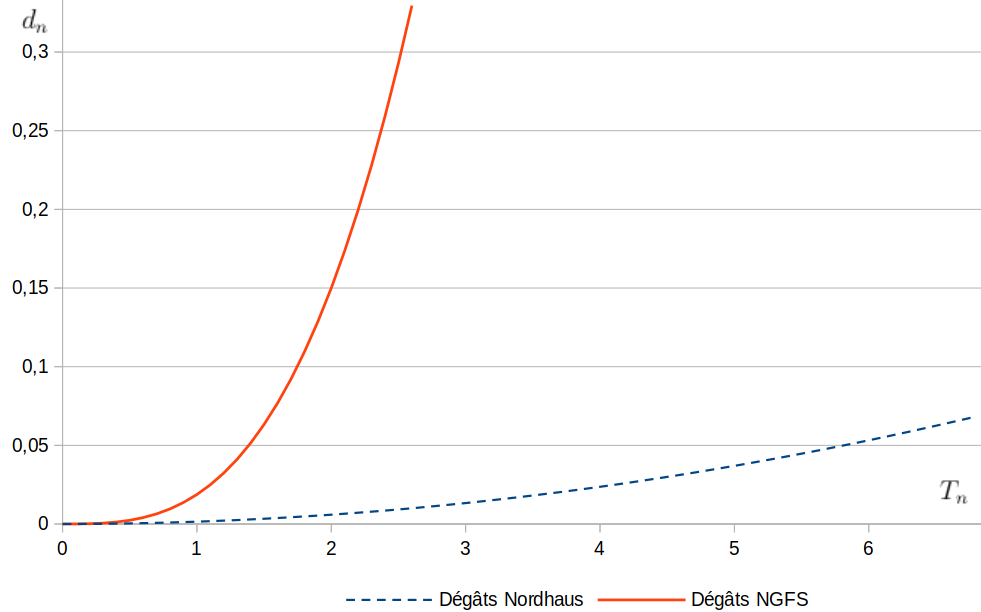
\includegraphics[scale=0.35]{images/fonction_degats.png}
\caption{Dégâts en fonction de la température}
\end{figure}

\section{Discussion et critiques}
\begin{enumerate}[resume]
\item Quelles variables sont endogènes, c'est-à-dire qu'elles sont calculées par le modèle ? Quelles variables sont exogènes, c'est-à-dire fixées par hypothèse grâce à des données d'autres études ?
\item Comment qualifier le modèle ? Top-down ou bottom-up ? Statique ou dynamique ? Stochastique ou déterministe ? Modèle d'optimisation ou non ? Discret ou continu ?
\item Comment améliorer ce modèle pour qu'ils décrivent mieux les liens entre économie et changement climatique ?
\item Quelles sont les simplifications que l'on a faites par rapport au modèle DICE du papier de Nordhaus de 1992 ?
\end{enumerate}


\end{document}